
\paragraph{The correctness of distributed algorithms} is the focus of this thesis. Distributed algorithms
are algorithms that are designed to run on multiple processors, without centralized control. They play a crucial role in modern computing.
For example, they control machines that we use on a daily basis such as smartphones, but also critical systems such as medical devices, trains, airplanes, and spaceships. Errors in distributed algorithms can have severe consequences, such as the loss of critical data or even the loss of human life. Ensuring their correctness is vital but challenging due to the inherent complexity of these systems~\cite{heiser2010theroad, lamport2019thebyzantine}. 

The Needham-Schroeder protocol~\cite{needham1978using}\textemdash a well-known distributed algorithm for two computers to verify each other's identity\textemdash exemplifies this challenge: it was found to have serious security flaws~\cite{lowe1996breaking} 17 years after it was published~\cite{cortier2014formal}.
To address the challenge of uncovering subtle vulnerabilities in distributed algorithms, one natural approach is to test all possible scenarios. This is effective when the number of scenarios is small, but becomes infeasible otherwise. For example, when there are infinitely many scenarios, program testing may reveal the presence of bugs, but is fundamentally incapable of demonstrating their absence.
This gap motivates the use of formal verification techniques\textemdash a family of mathematically rigorous methods for proving system correctness.

Formal verification techniques broadly fall into two categories: interactive theorem proving using proof assistants~\cite{moura2021lean4, bertot2004coq,nipkow2002isabelle} where humans guide proofs, and automated verification techniques~\cite{clarke2018model, contejean2011automated} for specific properties, which require minimal human intervention.

\paragraph{Automated verification techniques} are particularly interesting because they can be implemented as automated tools accessible to non-experts in formal verification while also accelerating verification for experts.
To verify a specific property of an algorithm, the user needs only to model the algorithm in a required formalism, and the tool then automatically checks conditions that mathematically imply the target property. To further ensure result correctness, advanced tools generate certificates verifiable by proof assistants~\cite{contejean2011automated}. 
Although theoretically incomplete for certain properties (meaning some inputs may yield no answer), well-designed techniques can handle many practical cases and significantly reduce verification effort.

This thesis focuses on developing automated verification techniques for distributed algorithms. 
To enable such methods, distributed algorithms must be modeled using a formalism that enables
rigorous analysis of their properties. We propose modeling states of distributed algorithms as edge-labeled directed multigraphs, algorithm behavior via graph transformation systems.

\paragraph{Finite edge-labeled directed multigraphs} generalize finite directed graphs by allowing multiple edges between nodes and labeled edges. Computation units are represented by nodes; communication channels are represented by edges; states of the system are modeled by graphs whose edges have labels representing information encoded in computation units and states of communication channels. For example, consider the graph $\mathcal{G}$ in~\autoref{fig:graph_modeling_state_network} enclosed in a box. It models a distributed network with six computation units.
 \begin{figure}[!htbp]
        \centering
        \resizebox{0.3\textwidth}{!}{
                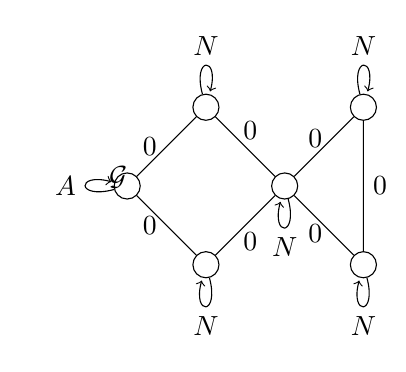
\begin{tikzpicture}
                    \graphbox{\( \mathcal{G} \)}{0mm}{0mm}{50mm}{50mm}{-10mm}{-25mm}{
                        \node[draw, circle] (n1) at (0,0) {};
                        \node[draw, circle] (n2) at (1,1) {};
                        \node[draw, circle] (n4) at (1,-1) {};
                        \node[draw, circle] (n3) at (2,0) {}; 
                        \node[draw, circle] (n5) at (3,-1){};
                        \node[draw, circle] (n6) at (3,1){};
                        \draw[-] (n1)--(n2)--(n3)--(n4);
                        \draw[-] (n4)--(n1);
                        \draw[-] (n3)--(n6)--(n5)--(n3);
                        \draw[transparent, rounded corners,rotate around={45:(0,-0.5)}, dotted] (0,-0.5) rectangle (2.2,0.3) ;
                        \draw[transparent, rounded corners,rotate around={-45:(0,0.5)}, dotted] (0,0.5) rectangle (2.2,-0.3) ;   
                        % \draw(-0.1,0) node[left] {A};
                        \draw[->] (n1) edge [loop left] node {$A$} (n1);
                        \draw[->] (n2) edge [loop above] node {$N$} (n2);
                        \draw[->] (n3) edge [loop below] node {$N$} (n3);
                        \draw[->] (n4) edge [loop below] node {$N$} (n4);
                        \draw[->] (n5) edge [loop below] node {$N$} (n5);
                        \draw[->] (n6) edge [loop above] node {$N$} (n6);
                        % \draw(1,1.1) node[above] {N};
                        % \draw(1,-1.1) node[below] {N};
                        % \draw(2,0.1) node[above] {N};
                        % \draw(3,1.1) node[above] {N};
                        % \draw(3,-1.1) node[below] {N};
                        % edge labels
                        \draw(1.35,0.7) node[right] {0};
                        \draw(1.35,-0.7) node[right] {0};
                        \draw(0.5,0.5) node[left] {0};
                        \draw(0.5,-0.5) node[left] {0};
                        \draw(2.6,0.6) node[left] {0};
                        \draw(2.6,-0.6) node[left] {0};
                        \draw(3,0) node[right] {0};
                    } 
                \end{tikzpicture} 
    }
    \caption{A graph modeling a network configuration}
    \label{fig:graph_modeling_state_network}
\end{figure}
Each node represents a computation unit, and a unit's state is indicated by the label of its self-loop edge.
 In~\autoref{fig:graph_modeling_state_network}, one unit is active ($A$) while the remaining five are neutral ($N$). Edges represent communication channels, all initially in state \textit{0}.

\paragraph{Graph transformation} provides an intuitive yet formal way to model distributed algorithms: state changes of the system are modeled by replacing subgraphs in the graph by other subgraphs according to transformation rules.
As an example, consider a distributed spanning tree construction algorithm: when an active unit ($A$) detects a neutral neighbor ($N$) via a channel in state \textit{0}, it activates the neighbor and updates the channel to state \textit{1}. Its behavior can be captured by a graph transformation rule illustrated in~\autoref{fig:intro:graph_transformation_rule_0}
% , denoted by $\mathcal{L} \to \mathcal{R}$, illustrated in~\autoref{fig:intro:graph_transformation_rule_0} where the graph is enclosed in a box with its name on the top left corner, numbers inside nodes are used to identify them. The rule operates as follows: it 
which
relabels the edges of an occurrence of the graph $\mathcal{L}$ in~\autoref{fig:intro:graph_transformation_rule_0} to obtain an occurrence of the graph $\mathcal{R}$ in~\autoref{fig:intro:graph_transformation_rule_0}.

% \tikz[baseline=0ex]{ 
%             \node (x) at (0,0) {$\bullet$};  
%             \node (y) at (1,0) {$\bullet$};
%             \draw[-] (x) -- node[midway,above] {$0$} (y) ;
%             % \node () at (0,0.3) {$A$};  
%             \draw[->] (x) edge [loop above] node {$A$} (x);
%             \draw[->] (y) edge [loop above] node {$N$} (y);
%             % \node () at (1,0.3) {$N$};
%  } then modifies its labels to obtain an occurrence of the graph \tikz[baseline=0ex]{ 
%                 \node (x) at (0,0) {$\bullet$};  
%                 \node (y) at (1,0) {$\bullet$};
%                 \draw[-] (x) -- node[midway,above] {$1$} (y) ;
%                 % \node () at (0,0.3) {$A$};  
%                 % \node () at (1,0.3) {$A$};
%                             \draw[->] (x) edge [loop above] node {$A$} (x);
%             \draw[->] (y) edge [loop above] node {$A$} (y);
%  }. It can be illustrated as~\autoref{fig:intro:graph_transformation_rule_0} where numbers inside nodes are their identifiers.
%  \begin{figure}[!htbp]
%     \centering
%     \begin{subfigure}{0.4\textwidth}
%        \begin{tikzpicture}
%                     \graphbox{\( \mathcal{L} \)}{0mm}{0mm}{34mm}{20mm}{-8mm}{-15mm}{
%                         \node[draw, circle] (x) at (0,0) {1};  
%                         \node[draw, circle] (y) at (2,0) {2};
%                         \draw[-] (x) -- node[midway,above] {$0$} (y) ;
%                         % \node  () at (0,0.5) {$A$};  
%                         % \node () at (2,0.5) {$N$};
%                                     \draw[->] (x) edge [loop above] node {$A$} (x);
%             \draw[->] (y) edge [loop above] node {$N$} (y);
%                     }
%        \end{tikzpicture}
%        \caption{Graph $\mathcal{L}$}
%        \label{fig:intro:graph_transformation_rule_l}
%     \end{subfigure}
%     \begin{subfigure}{0.4\textwidth}
%         \begin{tikzpicture}
%                     \graphbox{\( \mathcal{R} \)}{40mm}{0mm}{34mm}{20mm}{-8mm}{-15mm}{
%                         \node[draw, circle]  (x) at (0,0) {1};  
%                         \node[draw, circle]  (y) at (2,0) {2};
%                         \draw[-] (x) -- node[midway,above] {$1$} (y) ;
%                         % \node () at (0,0.5) {$A$};  
%                         % \node () at (2,0.5) {$A$};
%                         \draw[->] (x) edge [loop above] node {$A$} (x);
%                         \draw[->] (y) edge [loop above] node {$A$} (y);
%                     }  
%                     % \node () at (37mm,-10mm) {\( \rightarrow \)}; % K -> L
%                 \end{tikzpicture}
%                 \caption{Graph $\mathcal{R}$}
%              \label{fig:intro:graph_transformation_rule_r}
%         \end{subfigure}
%     \caption{}
%     \label{fig:intro:graph_transformation_rule_0}
% \end{figure}
    \begin{figure}[!htbp]
        \centering
        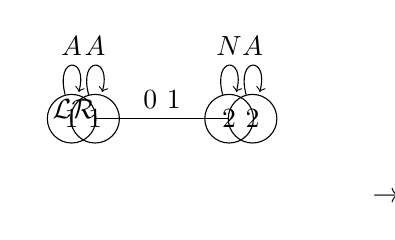
\begin{tikzpicture}
                    \graphbox{\( \mathcal{L} \)}{0mm}{0mm}{34mm}{20mm}{-8mm}{-15mm}{
                        \node[draw, circle] (x) at (0,0) {1};  
                        \node[draw, circle] (y) at (2,0) {2};
                        \draw[-] (x) -- node[midway,above] {$0$} (y) ;
                                    \draw[->] (x) edge [loop above] node {$A$} (x);
                        \draw[->] (y) edge [loop above] node {$N$} (y);
                    }
                    \graphbox{\( \mathcal{R} \)}{40mm}{0mm}{34mm}{20mm}{-8mm}{-15mm}{
                        \node[draw, circle]  (x) at (0,0) {1};  
                        \node[draw, circle]  (y) at (2,0) {2};
                        \draw[-] (x) -- node[midway,above] {$1$} (y) ;
                        \draw[->] (x) edge [loop above] node {$A$} (x);
                        \draw[->] (y) edge [loop above] node {$A$} (y);
                    }  
                    \node () at (37mm,-10mm) {\( \rightarrow \)}; % K -> L
        \end{tikzpicture}
        \caption{}
        \label{fig:intro:graph_transformation_rule_0}
    \end{figure}

A sample execution sequence starting from the configuration in~\autoref{fig:graph_modeling_state_network} is shown in~\autoref{fig:intro_sequence_of_transformation} where to improve readability, self-loops are omitted and their labels are displayed directly on nodes. 

Given an initial finite edge-labeled directed multigraph where all edges are labeled \textit{0} and all nodes are in the neutral state ($N$) except for a single node in the active state ($A$), when no further rule applications are possible, the subgraph induced by edges labeled \textit{1} constitutes a spanning tree.

    \begin{figure}[!htbp]
        \centering
        \resizebox{0.3\textwidth}{!}{
                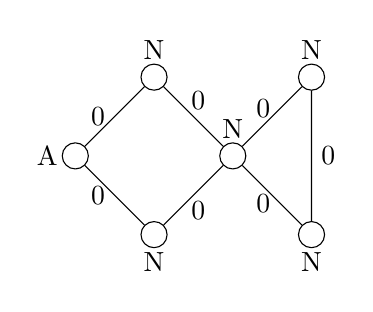
\begin{tikzpicture}
                    \node[draw, circle] (n1) at (0,0) {};
                    \node[draw, circle] (n2) at (1,1) {};
                    \node[draw, circle] (n4) at (1,-1) {};
                    \node[draw, circle] (n3) at (2,0) {};
                    \node[draw, circle] (n5) at (3,-1){};
                    \node[draw, circle] (n6) at (3,1){};
                    \draw[-] (n1)--(n2)--(n3)--(n4);
                    \draw[-] (n4)--(n1);
                    \draw[-] (n3)--(n6)--(n5)--(n3);
                    \draw[transparent, rounded corners,rotate around={45:(0,-0.5)}, dotted] (0,-0.5) rectangle (2.2,0.3) ;
                    \draw[transparent, rounded corners,rotate around={-45:(0,0.5)}, dotted] (0,0.5) rectangle (2.2,-0.3) ;   
    
                    \draw(-0.1,0) node[left] {A};
                    \draw(1,1.1) node[above] {N};
                    \draw(1,-1.1) node[below] {N};
                    \draw(2,0.1) node[above] {N};
                    \draw(3,1.1) node[above] {N};
                    \draw(3,-1.1) node[below] {N};
    
                    % edge labels
                    \draw(1.35,0.7) node[right] {0};
                    \draw(1.35,-0.7) node[right] {0};
                    \draw(0.5,0.5) node[left] {0};
                    \draw(0.5,-0.5) node[left] {0};
                    \draw(2.6,0.6) node[left] {0};
                    \draw(2.6,-0.6) node[left] {0};
                    \draw(3,0) node[right] {0};
                \end{tikzpicture}
    }
  \resizebox{0.3\textwidth}{!}{
                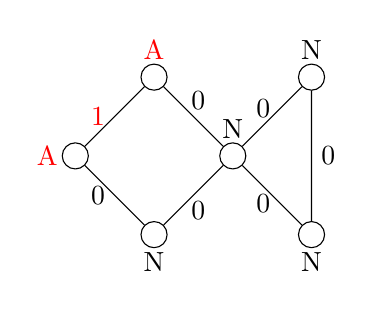
\begin{tikzpicture}
                    \node[draw, circle] (n1) at (0,0) {};
                    \node[draw, circle] (n2) at (1,1) {};
                    \node[draw, circle] (n4) at (1,-1) {};
                    \node[draw, circle] (n3) at (2,0) {};
                    
                    \node[draw, circle] (n5) at (3,-1){};
                    \node[draw, circle] (n6) at (3,1){};
        
                    \draw[-] (n1)--(n2)--(n3)--(n4);
                    \draw[-] (n4)--(n1);
                    \draw[-] (n3)--(n6)--(n5)--(n3);
        
                    \draw[transparent, rounded corners,rotate around={45:(0,-0.5)}, dotted] (0,-0.5) rectangle (2.2,0.3) ;
                    \draw[transparent, rounded corners,rotate around={-45:(0,0.5)}, dotted] (0,0.5) rectangle (2.2,-0.3) ;
    
                    \draw(-0.1,0) node[left] {\textcolor{red}{A}};
                    \draw(1,1.1) node[above] {\textcolor{red}{A}};
                    \draw(1,-1.1) node[below] {N};
                    \draw(2,0.1) node[above] {N};
                    \draw(3,1.1) node[above] {N};
                    \draw(3,-1.1) node[below] {N};
    
                    % edge labels
                    \draw(1.35,0.7) node[right] {0};
                    \draw(1.35,-0.7) node[right] {0};
                    \draw(0.5,0.5) node[left] {\textcolor{red}{1}};
                    \draw(0.5,-0.5) node[left] {0};
                    \draw(2.6,0.6) node[left] {0};
                    \draw(2.6,-0.6) node[left] {0};
                    \draw(3,0) node[right] {0};
                \end{tikzpicture}
}
\resizebox{0.3\textwidth}{!}{
                    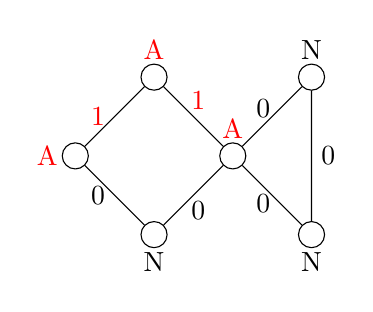
\begin{tikzpicture}
                        \node[draw, circle] (n1) at (0,0) {};
                        \node[draw, circle] (n2) at (1,1) {};
                        \node[draw, circle] (n4) at (1,-1) {};
                        \node[draw, circle] (n3) at (2,0) {};
                        
                        \node[draw, circle] (n5) at (3,-1){};
                        \node[draw, circle] (n6) at (3,1){};
            
                        \draw[-] (n1)--(n2)--(n3)--(n4);
                        \draw[-] (n4)--(n1);
                        \draw[-] (n3)--(n6)--(n5)--(n3);
            
                        \draw[transparent, rounded corners,rotate around={45:(0,-0.5)}, dotted] (0,-0.5) rectangle (2.2,0.3) ;
                        \draw[transparent, rounded corners,rotate around={-45:(0,0.5)}, dotted] (0,0.5) rectangle (2.2,-0.3) ;
    
                        \draw(-0.1,0) node[left] {\textcolor{red}{A}};
                        \draw(1,1.1) node[above] {\textcolor{red}{A}};
                        \draw(1,-1.1) node[below] {N};
                        \draw(2,0.1) node[above] {\textcolor{red}{A}};
                        \draw(3,1.1) node[above] {N};
                        \draw(3,-1.1) node[below] {N};
    
                        % edge labels
                        \draw(1.35,0.7) node[right] {\textcolor{red}{1}};
                        \draw(1.35,-0.7) node[right] {0};
                        \draw(0.5,0.5) node[left] {\textcolor{red}{1}};
                        \draw(0.5,-0.5) node[left] {0};
                        \draw(2.6,0.6) node[left] {0};
                        \draw(2.6,-0.6) node[left] {0};
                        \draw(3,0) node[right] {0};
                    \end{tikzpicture}
}


\resizebox{0.3\textwidth}{!}{
                    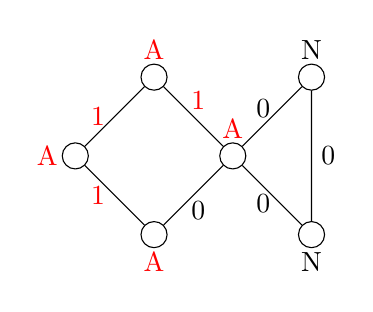
\begin{tikzpicture}
                        \node[draw, circle] (n1) at (0,0) {};
                        \node[draw, circle] (n2) at (1,1) {};
                        \node[draw, circle] (n4) at (1,-1) {};
                        \node[draw, circle] (n3) at (2,0) {};
                        
                        \node[draw, circle] (n5) at (3,-1){};
                        \node[draw, circle] (n6) at (3,1){};
            
                        \draw[-] (n1)--(n2)--(n3)--(n4);
                        \draw[-] (n4)--(n1);
                        \draw[-] (n3)--(n6)--(n5)--(n3);
            
                        \draw[transparent, rounded corners,rotate around={45:(0,-0.5)}, dotted] (0,-0.5) rectangle (2.2,0.3) ;
                        \draw[transparent, rounded corners,rotate around={-45:(0,0.5)}, dotted] (0,0.5) rectangle (2.2,-0.3) ;
    
                        \draw(-0.1,0) node[left] {\textcolor{red}{A}};
                        \draw(1,1.1) node[above] {\textcolor{red}{A}};
                        \draw(1,-1.1) node[below] {\textcolor{red}{A}};
                        \draw(2,0.1) node[above] {\textcolor{red}{A}};
                        \draw(3,1.1) node[above] {N};
                        \draw(3,-1.1) node[below] {N};
    
                        % edge labels
                        \draw(1.35,0.7) node[right] {\textcolor{red}{1}};
                        \draw(1.35,-0.7) node[right] {0};
                        \draw(0.5,0.5) node[left] {\textcolor{red}{1}};
                        \draw(0.5,-0.5) node[left] {\textcolor{red}{1}};
                        \draw(2.6,0.6) node[left] {0};
                        \draw(2.6,-0.6) node[left] {0};
                        \draw(3,0) node[right] {0};
                    \end{tikzpicture}
}
\resizebox{0.3\textwidth}{!}{
                    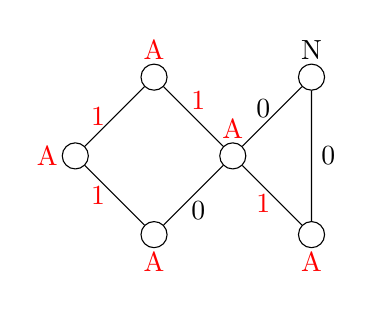
\begin{tikzpicture}
                        \node[draw, circle] (n1) at (0,0) {};
                        \node[draw, circle] (n2) at (1,1) {};
                        \node[draw, circle] (n4) at (1,-1) {};
                        \node[draw, circle] (n3) at (2,0) {};
                        
                        \node[draw, circle] (n5) at (3,-1){};
                        \node[draw, circle] (n6) at (3,1){};
            
                        \draw[-] (n1)--(n2)--(n3)--(n4);
                        \draw[-] (n4)--(n1);
                        \draw[-] (n3)--(n6)--(n5)--(n3);
            
                        \draw[transparent, rounded corners,rotate around={45:(0,-0.5)}, dotted] (0,-0.5) rectangle (2.2,0.3) ;
                        \draw[transparent, rounded corners,rotate around={-45:(0,0.5)}, dotted] (0,0.5) rectangle (2.2,-0.3) ;
              
                        \draw(-0.1,0) node[left] {\textcolor{red}{A}};
                        \draw(1,1.1) node[above] {\textcolor{red}{A}};
                        \draw(1,-1.1) node[below] {\textcolor{red}{A}};
                        \draw(2,0.1) node[above] {\textcolor{red}{A}};
                        \draw(3,1.1) node[above] {N};
                        \draw(3,-1.1) node[below] {\textcolor{red}{A}};
    
                        % edge labels
                        \draw(1.35,0.7) node[right] {\textcolor{red}{1}};
                        \draw(1.35,-0.7) node[right] {0};
                        \draw(0.5,0.5) node[left] {\textcolor{red}{1}};
                        \draw(0.5,-0.5) node[left] {\textcolor{red}{1}};
                        \draw(2.6,0.6) node[left] {0};
                        \draw(2.6,-0.6) node[left] {\textcolor{red}{1}};
                        \draw(3,0) node[right] {0};
                    \end{tikzpicture}
}
\resizebox{0.3\textwidth}{!}{
                    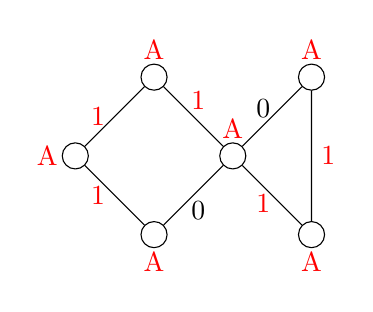
\begin{tikzpicture}
                        \node[draw, circle] (n1) at (0,0) {};
                        \node[draw, circle] (n2) at (1,1) {};
                        \node[draw, circle] (n4) at (1,-1) {};
                        \node[draw, circle] (n3) at (2,0) {};
                        
                        \node[draw, circle] (n5) at (3,-1){};
                        \node[draw, circle] (n6) at (3,1){};
            
                        \draw[-] (n1)--(n2)--(n3)--(n4);
                        \draw[-] (n4)--(n1);
                        \draw[-] (n3)--(n6)--(n5)--(n3);
            
                        \draw[transparent, rounded corners,rotate around={45:(0,-0.5)}, dotted] (0,-0.5) rectangle (2.2,0.3) ;
                        \draw[transparent, rounded corners,rotate around={-45:(0,0.5)}, dotted] (0,0.5) rectangle (2.2,-0.3) ;
                        \draw(-0.1,0) node[left] {\textcolor{red}{A}};
                        \draw(1,1.1) node[above] {\textcolor{red}{A}};
                        \draw(1,-1.1) node[below] {\textcolor{red}{A}};
                        \draw(2,0.1) node[above] {\textcolor{red}{A}};
                        \draw(3,1.1) node[above] {\textcolor{red}{A}};
                        \draw(3,-1.1) node[below] {\textcolor{red}{A}};
    
                        % edge labels
                        \draw(1.35,0.7) node[right] {\textcolor{red}{1}};
                        \draw(1.35,-0.7) node[right] {0};
                        \draw(0.5,0.5) node[left] {\textcolor{red}{1}};
                        \draw(0.5,-0.5) node[left] {\textcolor{red}{1}};
                        \draw(2.6,0.6) node[left] {0};
                        \draw(2.6,-0.6) node[left] {\textcolor{red}{1}};
                        \draw(3,0) node[right] {\textcolor{red}{1}};
                    \end{tikzpicture}
}
        \caption{Sequence of graph transformation}
        \label{fig:intro_sequence_of_transformation}
    \end{figure}

 Graph transformation has many applications, such as topology-based geometric modeling~\cite{poudret2007topology, belhaouari2014jerboa, bellet2017geometric, pascale2022Geometric_modeling}, DNA computing~\cite{harju2004tutorial_dna_computation}, and Software engineering~\cite{heckel2020software_engineers}.
 
 A predominant school of thought in this area is called algebraic graph rewriting~\cite{ehrig1997handbook1,ehrig1999handbook2,ehrig1999handbook3} which uses concepts from category theory~\cite{pierce1991basic,barr1990category,maclane2013categories} to define graph transformation. 
 The language of category theory abstracts away from the details of the different notions of graphs, provided that the notion of graph satisfies some properties~\cite{lack2004adhesive,overbeek2023graph}.  
This allows a uniform definition of graph transformation. In fact, there are different notions of graphs in the literature for different applications, such as edge-labeled multigraphs~\cite{konig2018atutorial,corradini1997algebraic}, hypergraphs~\cite{plump1993hypergraph}, attributed graphs~\cite{ehrig2006fundamentals}, etc. 
 Another advantage is that transformation is defined up to isomorphism. 
 This leads to an elegant definition of graph transformation. 

 Double-pushout (DPO) graph rewriting systems~\cite{corradini1997algebraic,habel2001double} are among the most studied algebraic graph transformation systems. A DPO graph rewriting rule consists of two functions that preserves graph structure $l:\mathcal{K} \to \mathcal{L}$ and $r:\mathcal{K} \to \mathcal{R}$, where $\mathcal{K}$ is called the interface graph, $\mathcal{L}$ is the left-hand side graph, and $\mathcal{R}$ is the right-hand side graph. As an example, consider the graph transformation rule in~\autoref{fig:intro:graph_transformation_rule_dpo} where graphs are enclosed in boxes with their names on the top left corner, numbers inside nodes are node identifiers.
  \begin{figure}[!htbp]
    \centering
    \begin{tikzpicture}
                    \graphbox{\( \mathcal{L} \)}{-40mm}{-3mm}{34mm}{15mm}{2mm}{2mm}{
                        \coordinate (o) at (0mm,-11mm); 
                        \node[draw,circle] (l1) at ($(o)+(-10mm,0mm)$) {1};
                        \node[draw,circle] (l2) at ($(l1)+(2,0)$) {2};
                        \node[draw,circle] (l3) at ($(l1) + (1,0)$) {3};
                        \draw[->] (l1) -- (l3) node[midway,above] {a};
                        \draw[->] (l3) -- (l2) node[midway,above] {a};
                    } 
                    \graphbox{\( \mathcal{K} \)}{0mm}{-3mm}{34mm}{15mm}{2mm}{2mm}{
                        \coordinate (o) at (0mm,-11mm); 
                        \node[draw,circle] (l1) at ($(o)+(-10mm,0mm)$) {1};
                        \node[draw,circle] (l2) at ($(l1)+(2,0)$) {2};
                    } 
                    \graphbox{\( \mathcal{R} \)}{40mm}{-3mm}{34mm}{15mm}{2mm}{2mm}{
                        \coordinate (o) at (0mm,-11mm); 
                        \node[draw,circle] (l1) at ($(o)+(-10mm,0mm)$) {1};
                        \node[draw,circle] (l2) at ($(l1)+(2,0)$) {2};
                    }  
                    \node () at (37mm,-10mm) {\( \overset{l}{\longrightarrow}\)}; % K -> L
                    \node () at (-3mm,-10mm) {\( \overset{r}{\longleftarrow}  \)}; % K -> L
                \end{tikzpicture}
    \caption{}
    \label{fig:intro:graph_transformation_rule_dpo}
\end{figure}
This rule identifies an occurrence of the graph \tikz[baseline=-0.5ex]{ 
        \node (x) at (0,0) {$\bullet$};  
        \node (y) at (1,0) {$\bullet$};
        \node (z) at (2,0) {$\bullet$};
        \draw[->] (x) -- node[midway,below] {a} (y) ;
        \draw[->] (y) -- node[midway,below] {a} (z) ;
}, and then removes the middle node and edges of the occurrence and adds no fresh nodes and edges. 

To apply a DPO graph rewriting rule $\mathcal{L} \overset{l}{\leftarrow} \mathcal{K} \overset{r}{\rightarrow} \mathcal{R}$ to a host graph $\mathcal{G}$, one must first identify an occurrence of $\mathcal{L}$ where a subgraph is called the interface graph. The other elements of the host graph $\mathcal{G}$ together with the interface graph form the context graph $\mathcal{C}$ of the rewriting step.
The graph $\mathcal{G}$ is thus decomposed into the occurrence of $\mathcal{L}$ and the context graph $\mathcal{C}$. 
Then, one
   modifies the occurrence of $\mathcal{L}$ (by removing some nodes and edges and adding some fresh nodes and edges while keeping the interface graph unchanged, and identifying nodes in the interface graph)
to obtain an occurrence of $R$.
   Finally, the result graph is obtained by gluing the occurrence of $\mathcal{R}$ with the context graph $\mathcal{C}$.


As an example, consider the graph $\mathcal{G}$ shown in~\autoref{fig:intro:graph_G}. 
It can be rewritten to the graph $\mathcal{H}$ shown in~\autoref{fig:intro:graph_H} by applying the DPO graph rewriting rule in~\autoref{fig:intro:graph_transformation_rule_dpo} on the unique occurrence of the graph $\mathcal{L}$.
Specifically,
the graph $\mathcal{G}$ can be decomposed, as shown in~\autoref{fig:intro:decomposition_of_G}, into the occurrence of the graph $\mathcal{L}$ (elements in orange and black) and the context graph $\mathcal{C}$ (elements in blue and black). The interface graph is the subgraph in black in~\autoref{fig:intro:decomposition_of_G}. The rule removes the orange part of the occurrence of $\mathcal{L}$ to obtain an occurrence of $\mathcal{R}$. 
The result graph $\mathcal{H}$ is obtained by gluing the occurrence of $\mathcal{R}$ and the context graph $\mathcal{C}$ via the interface graph.
  
\begin{figure}[!htbp]
    \centering
\begin{subfigure}{0.3\textwidth}
   \centering
  \begin{tikzpicture}
     \graphbox{\( \mathcal{G} \)}{0mm}{-22mm}{34mm}{22mm}{2mm}{-3mm}{
              \coordinate (o) at (0mm,-3mm); 
              \node[draw,circle] (l1) at ($(o)+(-10mm,0mm)$) {1};
              \node[draw,circle] (l2) at ($(l1)+(2,0)$) {2};
              \node[draw,circle] (l3) at ($(l1) + (1,0)$) {3};
              \node[draw,circle] (l4) at ($(l2) + (0,-1)$) {6};
              \draw[] (l1) -- (l3) node[midway,above] {a};
              \draw[] (l3) -- (l2) node[midway,above] {a};
              \draw[ ] (l2) -- (l4) node[midway,right] {b};
              \node[draw,circle] (l6) at ($(l1) + (0,-1)$) {7};
              \draw[] (l1) -- (l6) node[midway,left] {b};
          }  
  \end{tikzpicture}
  \caption{Graph $\mathcal{G}$}
  \label{fig:intro:graph_G}
\end{subfigure}
  \begin{subfigure}{0.3\textwidth}
   \centering  
   \begin{tikzpicture}
          \graphbox{\( \mathcal{H} \)}{40mm}{-22mm}{34mm}{22mm}{2mm}{-3mm}{
              \coordinate (o) at (0mm,-3mm); 
              \node[draw,circle] (l1) at ($(o)+(-10mm,0mm)$) {1};
              \node[draw,circle] (l2) at ($(l1)+(2,0)$) {2};
              \node[draw,circle] (l4) at ($(l2) + (0,-1)$) {6};
              \draw[ ] (l2) -- (l4) node[midway,right] {b};
              \node[ draw,circle] (l6) at ($(l1) + (0,-1)$) {7};
              \draw[ ] (l1) -- (l6) node[midway,left] {b};
          }    
  \end{tikzpicture}
  \caption{Graph $\mathcal{H}$}
  \label{fig:intro:graph_H}
\end{subfigure}
\begin{subfigure}{0.3\textwidth}
   \centering
  \begin{tikzpicture}
     \graphbox{\( \mathcal{G} \)}{0mm}{-22mm}{34mm}{22mm}{2mm}{-3mm}{
              \coordinate (o) at (0mm,-3mm); 
              \node[draw,circle] (l1) at ($(o)+(-10mm,0mm)$) {1};
              \node[draw,circle] (l2) at ($(l1)+(2,0)$) {2};
              \node[orange,draw,circle] (l3) at ($(l1) + (1,0)$) {3};
              \node[blue,draw,circle] (l4) at ($(l2) + (0,-1)$) {6};
              \draw[orange] (l1) -- (l3) node[midway,above] {a};
              \draw[orange] (l3) -- (l2) node[midway,above] {a};
              \draw[blue] (l2) -- (l4) node[midway,right] {b};
              \node[blue,draw,circle] (l6) at ($(l1) + (0,-1)$) {7};
              \draw[blue] (l1) -- (l6) node[midway,left] {b};
          }  
  \end{tikzpicture}
  \caption{Decomposition of $\mathcal{G}$}
  \label{fig:intro:decomposition_of_G}
\end{subfigure}
    \caption{}
\end{figure}

A DPO rewriting rule cannot always be applied to a graph with an occurrence of the left-hand side graph.
For example, consider the rule in~\autoref{fig:intro:graph_transformation_rule_dpo} and the graph $\mathcal{G}'$ in~\autoref{fig:intro:dangling_edge} which is obtained from the graph $\mathcal{G}$ in~\autoref{fig:intro:graph_G} by adding an edge from node 3 to node 6 (in red). This graph has the same occurrence of the left-hand side graph $\mathcal{L}$ as the graph $\mathcal{G}$ in~\autoref{fig:intro:graph_G}. However, when the node 3 is removed, the edge from node 3 to node 6 becomes dangling.

\begin{figure}[!htbp]
   \centering
  \begin{tikzpicture}
    \graphbox{\( \mathcal{G}' \)}{0mm}{-22mm}{34mm}{22mm}{2mm}{-3mm}{
                \coordinate (o) at (0mm,-3mm); 
                \node[draw,circle] (l1) at ($(o)+(-10mm,0mm)$) {1};
                \node[draw,circle] (l2) at ($(l1)+(2,0)$) {2};
                \node[draw,circle] (l3) at ($(l1) + (1,0)$) {3};
                \node[draw,circle] (l4) at ($(l2) + (0,-1)$) {6};
                \draw[->,red] (l3) -- (l4) node[midway,above] {b};
                \draw[->] (l1) -- (l3) node[midway,above] {a};
                \draw[->] (l3) -- (l2) node[midway,above] {a};
                \draw[->] (l2) -- (l4) node[midway,right] {b};
                \node[draw,circle] (l6) at ($(l1) + (0,-1)$) {7};
                \draw[<-] (l1) -- (l6) node[midway,left] {b};
                % \draw[->] (l2) edge[out=-135,in=-45]node[midway,below] {a} (l1) ;
            }   
  \end{tikzpicture}
  \caption{}
  \label{fig:intro:dangling_edge}
\end{figure}
DPO graph rewriting forbids transformations causing dangling edges. Nevertheless,
in the literature, different ways of handling dangling edges have been proposed which 
lead to different algebraic graph rewriting systems.
  Some formalisms, such as single pushout (SPO) graph rewriting systems~\cite{ehrig1997algebraic}, allow transformations causing dangling edges and implicitly remove them. Others such as AGREE~\cite{corradini2015agree}, PBPO~\cite{corradini2019thepbpo}, PBPO+~\cite{overbeek2023graph} graph rewriting systems provides mechanisms for each rule to impose restrictions on the context graph.

   We focus on DPO graph rewriting systems in this thesis for three reasons.
   Firstly, it is among the most studied algebraic graph rewriting formalisms, which means a large potential user base for our automated techniques.
   Secondly, its relative simplicity stems from relying solely on the concept of pushouts~\cite{pierce1991basic} which minimizes the categorical prerequisites required to understand it. This is interesting because the abstract nature of category theory is often seen as a barrier to entry for newcomers~\cite{overbeekthesis}.
    Finally, despite its conceptual simplicity, DPO graph rewriting systems remain sufficiently expressive to model many distributed algorithms.
    For example, the transformation rules in~\autoref{fig:intro:graph_transformation_rule_0} can be expressed as DPO graph transformation rules as in~\autoref{fig:intro:graph_transformation_rule_dpo} and~\autoref{fig:intro:graph_transformation_rule_0_dpo} respectively.
  
     \begin{figure}[!htbp]
    \centering
       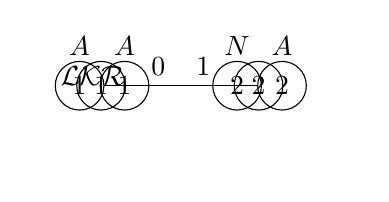
\begin{tikzpicture} 
                    \graphbox{\( \mathcal{L} \)}{-40mm}{-3mm}{34mm}{15mm}{-8mm}{-9mm}{
                        \node[draw, circle] (x) at (0,0) {1};  
                        \node[draw, circle] (y) at (2,0) {2};
                        \draw[-] (x) -- node[midway,above] {0} (y) ;
                        \node  () at (0,0.5) {$A$};  
                        \node () at (2,0.5) {$N$};
                    } 
                    \graphbox{\( \mathcal{K} \)}{0mm}{-3mm}{34mm}{15mm}{-8mm}{-9mm}{
                        \node[draw, circle] (x) at (0,0) {1};  
                        \node[draw, circle] (y) at (2,0) {2};
                    } 
                    \graphbox{\( \mathcal{R} \)}{40mm}{-3mm}{34mm}{15mm}{-8mm}{-9mm}{
                        \node[draw, circle] (x) at (0,0) {1};  
                        \node[draw, circle] (y) at (2,0) {2};
                        \draw[-] (x) -- node[midway,above] {1} (y) ;
                        \node  () at (0,0.5) {$A$};  
                        \node () at (2,0.5) {$A$};
                    }  
                    \node () at (37mm,-10mm) {\( \rightarrowtail \)}; % K -> L
                    \node () at (-3mm,-10mm) {\( \leftarrowtail  \)}; % K -> L
                \end{tikzpicture}
    \caption{}
    \label{fig:intro:graph_transformation_rule_0_dpo}
    \end{figure}
    
Since graph transformation rules in a system are applied repeatedly and nondeterministically, they can lead to infinite sequences of graph transformations. However, some properties of systems dependent on the absence of infinite sequences. For example, the transformation system in~\autoref{fig:intro:graph_transformation_rule_0} can construct a spanning tree of a connected graph with edges and nodes labeled as required, if the transformation system terminates. It is thus crucial to ensure that a rewriting system terminates.

\paragraph{Termination} is a property of algorithms which ensures that they eventually halt. In the context of DPO graph rewriting systems, it ensures that no graph can be transformed indefinitely under a given set of rewriting rules. 
For example, the rule in~\autoref{fig:intro:graph_transformation_rule_dpo} terminates because each application reduces the number of nodes in a graph by one. For an example of a rewriting rule which does not terminate, consider the rewriting rule in~\autoref{fig:intro:graph_transformation_rule_nonterminating}. 
\begin{figure}[!htbp]
        \centering
            \resizebox{0.85\textwidth}{!}{
                \begin{tikzpicture}[baseline=-3ex]
                    \graphbox{\( \mathcal{L} \)}{0mm}{-3mm}{34mm}{15mm}{2mm}{2mm}{
                        \coordinate (o) at (0mm,-11mm); 
                        \node[draw,circle] (l1) at ($(o)+(-10mm,0mm)$) {1};
                        \node[draw,circle] (l2) at ($(l1)+(2,0)$) {2};
                        \node[draw,circle] (l3) at ($(l1) + (1,0)$) {3};
                        \draw[->] (l1) -- (l3) node[midway,above] {a};
                        \draw[->] (l3) -- (l2) node[midway,above] {b};
                    } 
            
                    \graphbox{\( \mathcal{K} \)}{40mm}{-3mm}{34mm}{15mm}{2mm}{2mm}{
                        \coordinate (o) at (0mm,-11mm); 
                        \node[draw,circle] (l1) at ($(o)+(-10mm,0mm)$) {1};
                        \node[draw,circle] (l2) at ($(l1)+(2,0)$) {2};
                    }  
            
                    \graphbox{\( \mathcal{R} \)}{80mm}{-3mm}{35mm}{13mm}{5mm}{2mm}{
                        \coordinate (o) at (-5mm,-11mm); 
                        \node[draw,circle] (l1) at ($(o)+(-10mm,0mm)$) {1};
                        % \node[draw,circle] (l2) at ($(l1)+(3,0)$) {2};
                        \node[draw,circle] (l3) at ($(l1) + (1,0)$) {4};
                        \node[draw,circle] (l4) at ($(l1) + (2,0)$) {2};
                        \draw[->] (l1) -- (l3) node[midway,above] {b};
                        \draw[->] (l3) -- (l4) node[midway,above] {a};
                        % \draw[->] (l4) -- (l2) node[midway,above] {a};
                    }    
                    \node () at (37mm,-10mm) {\( \leftarrowtail \)}; % K -> L
                    \node () at (77mm,-10mm) {\( \rightarrowtail \)}; % K -> R
                \end{tikzpicture}
                }
        \caption{}
        \label{fig:intro:graph_transformation_rule_nonterminating}
    \end{figure}
It replaces an occurrence of the graph \tikz[baseline=-0.5ex]{ 
        \node (x) at (0,0) {$\bullet$};  
        \node (y) at (1,0) {$\bullet$};
        \node (z) at (2,0) {$\bullet$};
        \draw[->] (x) -- node[midway,below] {a} (y) ;
        \draw[->] (y) -- node[midway,below] {b} (z) ;
} by that of the graph \tikz[baseline=-0.5ex]{ 
        \node (x) at (0,0) {$\bullet$};  
        \node (y) at (1,0) {$\bullet$};
        \node (z) at (2,0) {$\bullet$};
        \draw[->] (x) -- node[midway,below] {b} (y) ;
        \draw[->] (y) -- node[midway,below] {a} (z) ;
} while keeping the extreme nodes unchanged.
    A looping rewriting sequence using this rule can be constructed as shown in~\autoref{fig:intro:sequence_of_transformation_infinite}.

        \begin{figure}[!htbp]
            \centering
          \resizebox{0.85\textwidth}{!}{
            \tikz
            [baseline=-0.5ex]
            { 
                \node (x) at (0,0) {$\bullet$};  
                \node (y) at (1,0) {$\bullet$};
                \node (z) at (0.5,0.86) {$\bullet$};
                \draw[->,red] (x) -- node[midway,below] {a} (y) ;
                \draw[->,red] (y) -- node[midway,right] {b} (z) ;
                \draw[->] (z) -- node[midway,left] {b} (x) ;
            } 
            $\Rightarrow$ 
            \tikz[baseline=-0.5ex]{ 
                \node (x) at (0,0) {$\bullet$};  
                \node (y) at (1,0) {$\bullet$};
                \node (z) at (0.5,0.86) {$\bullet$};
                \draw[->] (x) -- node[midway,below] {b} (y) ;
                \draw[->,red] (y) -- node[midway,right] {a} (z) ;
                \draw[->,red] (z) -- node[midway,left] {b} (x) ;
            }
            $\Rightarrow$ 
            \tikz[baseline=-0.5ex]{ 
                \node (x) at (0,0) {$\bullet$};  
                \node (y) at (1,0) {$\bullet$};
                \node (z) at (0.5,0.86) {$\bullet$};
                \draw[->,red] (x) -- node[midway,below] {b} (y) ;
                \draw[->] (y) -- node[midway,right] {b} (z) ;
                \draw[->,red] (z) -- node[midway,left] {a} (x) ;
            }
            $\Rightarrow$ 
            \tikz[baseline=-0.5ex]{ 
                \node (x) at (0,0) {$\bullet$};   
                \node (y) at (1,0) {$\bullet$};
                \node (z) at (0.5,0.86) {$\bullet$};
                \draw[->,red] (x) -- node[midway,below] {a} (y) ;
                \draw[->,red] (y) -- node[midway,right] {b} (z) ;
                \draw[->] (z) -- node[midway,left] {b} (x) ;
            }
          }
          \caption{}
          \label{fig:intro:sequence_of_transformation_infinite}
        \end{figure}

Many termination techniques exist for term rewriting systems~\cite{nipkow1998term, dershowitz1982orderings, middeldorp1997simple, arts2000termination}.  
Most exploit the tree structure of terms—a feature absent in general graphs—making direct adaptation impossible. 
% ,dick1990automating,giesl1995generating,zantema1994termination,bellegarde1990termination,zantema1995termination
% These techniques prove the termination of a rewriting system by embedding the binary relations defined by a term rewriting system onto a well-founded order. This is done either explicitly or implicitly. 
% In the cases, for example , one defines explicitly a well-founded order on terms, and then proves that terms can be interpreted as elements of the well-founded order, and that the application of a rule transforms a term into another term that is smaller than the original term in the well-founded order~\cite{.
% In the latter case, one defines a well-founded order on terms, and then proves that the application of a rule transforms a term into another term that is smaller than the original term in the well-founded order. In this case,
% the technique is classified as \enquote{techniques by interpretation} in the literature, and in the latter case, they are classified as \enquote{syntactic techniques}, \enquote{techniques by dependencies pairs}, \enquote{semantic labelling}, \enquote{hierarchical termination}, etc. \todo{references and explanation}
Therefore, new techniques are needed for proving termination of DPO graph rewriting systems. 

% However, developing termination techniques for rewriting systems is difficult, because a system may have many rules, and, therefore, many constraints on the behavior of the rules must be satisfied. A more interesting approach is to prove that the system in question can be separated into two disjoint subsets of rules, one of which can be applied only finitely many times in any sequence using rules from the union of the two sets, thus the termination of the system can be reduced to the termination of the other set of rules. 
However, the concept of termination is too restrictive in the context of rewriting systems. Consider the graph transformation system with two rules illustrated in~\autoref{fig:intro:edge_deletion_and_node_addition_rule}: rule $\alpha$ deletes an arbitrary edge labeled by $A$ and rule $\beta$ introduces a fresh node.
  \begin{figure}[!htbp]
        \centering
%   \begin{subfigure}{0.3\textwidth}
%         % \centering
        $\alpha$ = {
             \resizebox{0.7\textwidth}{!}{
             \begin{tikzpicture}[baseline=-7ex]
                    \graphbox{\( \mathcal{L} \)}{0mm}{-3mm}{34mm}{15mm}{2mm}{2mm}{
                        \coordinate (o) at (0mm,-11mm); 
                        \node[draw,circle] (l1) at ($(o)+(-10mm,0mm)$) {1};
                        \node[draw,circle] (l2) at ($(l1)+(2,0)$) {2};
                        \draw[->] (l1) -- (l2) node[midway,above] {A};
                    } 
            
                    \graphbox{\( \mathcal{K} \)}{40mm}{-3mm}{34mm}{15mm}{2mm}{2mm}{
                        \coordinate (o) at (0mm,-11mm); 
                        \node[draw,circle] (l1) at ($(o)+(-10mm,0mm)$) {1};
                        \node[draw,circle] (l2) at ($(l1)+(2,0)$) {2};
                    }  
            
                    \graphbox{\( \mathcal{R} \)}{80mm}{-3mm}{35mm}{15mm}{5mm}{2mm}{
                        \coordinate (o) at (-5mm,-11mm); 
                        \node[draw,circle] (l1) at ($(o)+(-10mm,0mm)$) {1};
                        \node[draw,circle] (l4) at ($(l1) + (2,0)$) {2};
                    }    
                    \node () at (37mm,-10mm) {\( \leftarrowtail \)}; % K -> L
                    \node () at (77mm,-10mm) {\( \rightarrowtail \)}; % K -> R
                \end{tikzpicture}
            }
        }
    %     \caption{A graph transformation rule for edge deletion}
    % \label{fig:intro:edge_deletion_rule}
    % \end{subfigure}
    
    % \begin{subfigure}{0.3\textwidth}
    %     % \centering

        $\beta$ ={
             \resizebox{0.7\textwidth}{!}{
             \begin{tikzpicture}[baseline=-7ex]
                    \graphbox{\( \mathcal{L} \)}{0mm}{-3mm}{34mm}{15mm}{2mm}{2mm}{
                        
                    } 
            
                    \graphbox{\( \mathcal{K} \)}{40mm}{-3mm}{34mm}{15mm}{2mm}{2mm}{
                       
                    }  
            
                    \graphbox{\( \mathcal{R} \)}{80mm}{-3mm}{35mm}{15mm}{5mm}{2mm}{
                        \coordinate (o) at (0mm,-11mm); 
                        \node[draw,circle] (l1) at ($(o)+(-10mm,0mm)$) {};
                    }    
                    \node () at (37mm,-10mm) {\( \leftarrowtail \)}; % K -> L
                    \node () at (77mm,-10mm) {\( \rightarrowtail \)}; % K -> R
                \end{tikzpicture}
            }
        }
    %     \caption{A graph transformation rule for node addition}
    %     \label{fig:intro:node_addition_rule}
    % \end{subfigure}
    \caption{A rewriting system}
    \label{fig:intro:edge_deletion_and_node_addition_rule}
  \end{figure}
  This system does not terminate, as the node-adding rule $\beta$ can be applied indefinitely. Yet, in any sequence of graph transformation with this system, rule $\alpha$ can only be applied finitely many times, because it removes an edge from the graph, and the initial graph is finite. Thus, the termination of the system can be established if the system with the unique rule $\beta$ terminates (which is not termination). This observation leads to the concept of relative termination.

\paragraph{Relative termination} is a concept introduced by Klop in~\cite{klop1987term} for binary relations. It can be adapted to the context of rewriting systems because the relation \enquote{Graph X can be rewritten to graph Y by a sequence of rule application} is a binary relation. In the context of rewriting systems, it can be formalized as follows:
 given two rule sets \( \mathcal{A} \) and \( \mathcal{B} \), \( \mathcal{A} \) is relatively terminating with respect to \( \mathcal{B} \) if for any finite graph $G$,
rules in $\mathcal{A}$ can only be applied finitely many times in any sequence of rule applications from $\mathcal{A} \cup \mathcal{B}$. In the case where a set of rule $\mathcal{R}$ can be partitioned into two disjoint subsets \( \mathcal{A} \) and \( \mathcal{B} \), if \( \mathcal{A} \) is relatively terminating with respect to \( \mathcal{B} \), then the termination of the rewriting system with rules in \( \mathcal{R} \) can be reduced to the termination of the rewriting system with only the rules in \( \mathcal{B} \). When \( \mathcal{B} \) is the empty set, the termination of the rewriting system with rules in \( \mathcal{R} \) can be concluded, because a system without rules terminates.
This concept has been applied in some previous work on termination of DPO graph rewriting systems~\cite{zantema2014termination,bruggink2014termination,bruggink2015proving,endrullis2024generalized_icgt}.

  
  % This concept has been applied in some previous work on termination of DPO graph rewriting systems~\cite{bruggink2014termination,bruggink2015proving}. 
  % It can be used to simplify the termination analysis of a rewriting system. 
  % Specifically, given a rewriting system with two rule sets \( \mathcal{A} \) and \( \mathcal{B} \), if \( \mathcal{A} \) is relatively terminating with respect to \( \mathcal{B} \), then the termination of the rewriting system can be reduced to the termination of the rewriting system with only the rules in \( \mathcal{B} \). 
  % Therefore, if we can prove that a rule set is relatively terminating with respect to another rule set, we can reduce the problem of proving termination of the union of the two rule sets to proving termination of one of them.
% Intuitively, this property corresponds to the phenomenon that while some distributed systems do not halt for every input, some of their operations can only be applied finitely many times in any execution. 
% Therefore, these operations do not need to be considered when reasoning about the termination of the system. The problem to be analyzed can thus be simplified by safely ignoring these operations.
  This approach has several advantages.
  Firstly, by successful elimination of irrelevant rules, it allows us to localize the essential part of a rewriting system to termination analysis.
  Secondly, different techniques can cooperate in a straightforward way, leveraging the strengths of each technique, because at each iteration of the analysis, we can try different techniques.
   Thirdly, combined with Plump's modular termination technique~\cite{plump2018modular}, which proves termination of a system by establishing termination for two rule sets that partition the system's rules, the termination analysis of DPO graph rewriting systems can be much easier.

\paragraph{Termination of DPO graph rewriting systems on edge-labeled directed multigraphs} is the focus of this thesis, even though, using the language of category theory, it is possible to develop termination techniques for DPO rewriting systems on different graph notions that satisfy certain properties. There are several reasons for this choice.

First of all, edge-labeled directed multigraphs are simple and intuitive: they are just directed graphs with multiple edges between two nodes allowed, and each edge is labeled by a symbol from a finite alphabet. This notion of graph is widely used in the literature, such as in the work introducing the DPO graph rewriting~\cite{ehrig1973graph}, in previous work on the method that we extend in~\autoref{chap:nwf}~\cite{bruggink2014termination,bruggink2015proving,zantema2014termination}, and in illustrative examples of works~\cite{overbeek2024termination_lmcs,endrullis2024generalized_icgt} which are closely related to our work in~\autoref{chap:subgraph_counting} and~\autoref{chap:antipattern}.

 Secondly, by focusing on this notion of graph, we want to avoid overly abstract reasoning and make the techniques more accessible to users than those based on more abstract notions of graph, such as adhesive categories~\cite{lack2004adhesive}.
 As a consequence, the correctness of our technique in~\ref{chap:subgraph_counting} and~\ref{chap:antipattern} can be checked easily by users with basic knowledge in graph theory and very basic knowledge in category theory.

Finally, specializing to edge-labeled directed multigraphs enables us to leverage graph-specific properties to develop stronger termination criteria. Because termination is undecidable for general DPO graph rewriting systems~\cite{plump1998terminationundecidable}, this specialization is essential for extending the boundaries of practically verifiable termination. 

\paragraph{Existing techniques}
Few techniques for proving (relative) termination of DPO graph rewriting systems exist. Below, we list some of the existing techniques.

\begin{itemize}
    \item Overbeek and Endrullis developed a termination technique for PBPO+ graph rewriting systems~\cite{overbeek2024termination_lmcs}. This technique counts the number of occurrences of certain subgraphs before and after a rewriting step. This technique can be applied to PBPO+ graph rewriting systems on many categories including edge-labeled directed multigraphs. It can also be applied to left-injective DPO graph rewriting systems.
    \item The type graph method, which weighs an object by summing the weights of morphisms from the object to a type graph, was initially introduced by Zantema, K{\"o}nig and Bruggink~\cite{zantema2014termination} for cycle-rewriting systems. 
    This method has since been generalized to edge-labeled multigraphs by Bruggink et al.~\cite{bruggink2014termination} for DPO rewriting with monic matches and injective rules, later extended to DPO rewriting in general by Bruggink et al.~\cite{bruggink2015proving}, and further adapted to more categories and different DPO variants by Endrullis et al.~\cite{endrullis2024generalized_arxiv_v2}. 
    \item Plump~\cite{plump1995ontermination} introduced a necessary and sufficient termination condition for left-injective DPO hypergraph rewriting via forward closure, though verifying this condition is undecidable. 
    \item Plump~\cite{plump2018modular} later proposed a modular critical pair-based strategy for left-injective DPO hypergraph rewriting with monic matches. It allows to deduce termination of the union of two systems from the termination of their sub-systems.
    % \item Levendovszky et al.~\cite{levendovszky2007termination} propose a termination criterion for DPO rewriting (monic matches, injective rules, negative application condition), though automated verification is hard as explained in~\cite[\textsection 6]{levendovszky2007termination}. 
    % \item Bottoni et al.~\cite{bottoni2005termination} propose a termination criterion for DPO/SPO rewriting on high-level replacement units. Their method imposes a strongly constrained measuring function and the only concretes measuring function proposed are node-counting and edge-counting.
    % \item Bottoni et al.~\cite{bottoni2010atermination} present a criterion for termination of DPO rewriting with monic matches, injective rules and negative application conditions, based on the construction of a labeled transition system. 
\end{itemize}

\paragraph{Contribution 1: Termination of Graph Rewriting Using Weighted Type Graphs over Non-well-founded Semirings}

While the weighted type graph method is a powerful technique for proving termination of double-pushout (DPO) graph rewriting systems, existing approaches require weighted type graphs to have weights over well-founded semirings. This approach has practical limitations when applied to edge-labeled directed multigraph rewriting. Chapter~\ref{chap:nwf} investigates the use of non-well-founded semirings to overcome these limitations. 
% Chapter~\ref{chap:nwf} is based on the following paper:
% \begin{itemize}
%     \item Qi Qiu. Termination of Graph Rewriting using Weighted Type Graphs over Non-well-founded Semirings. 16th International Workshop on Graph Computation Models, Jun 2025, Koblenz, Germany. 2025. ⟨hal-04954960v3⟩
% \end{itemize}
 
\paragraph{Contribution 2: Termination of Injective DPO Graph Rewriting Systems Using Subgraph Counting} 

To resolve some cases that prior interpretation-based methods cannot handle, Chapter~\ref{chap:subgraph_counting} presents a new machine-checkable sufficient condition for relative termination of DPO graph rewriting systems with injective rules on edge-labeled multigraphs. 
It is based on the idea that if the number of a specific subgraph in the graph strictly decreases every time a transformation is performed, then the transformation cannot last indefinitely.
The method defines a graph's weight as the sum of weights of occurrences of a set of graphs within it. Given two rule sets $A$ and $B$, by ensuring 
(1) every rewriting step using rules in $A$ strictly decreases the host graph's weight and 
(2) every rewriting step using rules in $B$ never increases it, we guarantee that rules in $A$ can be applied only finitely many times in any rewriting sequence using rules from the union of $A$ and $B$. 
% Chapter~\ref{chap:subgraph_counting} is based on the following paper:
% \begin{itemize}
%     \item Qiu, Q. (2025). Termination of Injective DPO Graph Rewriting Systems Using Subgraph Counting. In: Endrullis, J., Tichy, M. (eds) Graph Transformation. ICGT 2025. Lecture Notes in Computer Science, vol 15720. Springer, Cham. \url{https://doi.org/10.1007/978-3-031-94706-3_1}
% \end{itemize}

\paragraph{Contribution 3: Termination of Injective DPO Graph Rewriting Systems Using Subgraph Counting with Antipattern}

The termination property of a graph rewriting system can sometimes be established by analyzing a decrease in the number of occurrences of specific subgraphs that are not embedded within forbidden contexts. For example, consider the DPO graph rewriting rule in~\autoref{fig:intro:graph_transformation_rule_anti_pattern}.
 \begin{figure}[!htbp]
    \centering
\begin{tikzpicture}
      \graphbox{$L$}{0mm}{0mm}{34mm}{20mm}{2mm}{-5mm}{
          \coordinate (o) at (0mm,-3mm); 
          \node[draw,circle] (l1) at ($(o)+(-10mm,0mm)$) {1};
          \node[draw,circle] (l2) at ($(l1)+(2,0)$) {2};
          \node[draw,circle] (l3) at ($(l1) + (1,0)$) {3};
          \draw[->] (l1) -- (l3) node[midway,above] {a};
          \draw[->] (l3) -- (l2) node[midway,above] {a};
      }     
      \graphbox{$K$}{40mm}{0mm}{24mm}{20mm}{2mm}{-5mm}{
          \coordinate (o) at (5mm,-3mm); 
          \node[draw,circle] (l1) at ($(o)+(-10mm,0mm)$) {1};
          \node[draw,circle] (l2) at ($(l1)+(1,0)$) {2};
      }    
      \graphbox{$R$}{70mm}{0mm}{45mm}{20mm}{2mm}{-5mm}{
        \coordinate (o) at (0mm,-3mm); 
        \node[draw,circle] (l1) at ($(o)+(-10mm,0mm)$) {1};
        \node[draw,circle] (l2) at ($(l1)+(2,0)$) {2};
        \node[draw,circle] (l3) at ($(l1) + (1,0)$) {3};
        \draw[->] (l1) -- (l3) node[midway,above] {a};
        \draw[->] (l3) -- (l2) node[midway,above] {a};
        \draw[->] (l3) edge [loop below] node {$c$} (l3);
      }    

      \node () at (37mm,-10mm) {$\leftarrowtail$};
      \node () at (67mm,-10mm) {$\rightarrowtail$};
  \end{tikzpicture}
  \caption{}
  \label{fig:intro:graph_transformation_rule_anti_pattern}
 \end{figure}

 
Each application of this rule reduces the number of occurrences of the left-hand side graph $L$ that are not included in any occurrence of the right-hand side graph $ R $. While this variant suggests termination, existing subgraph counting methods (e.g., those in Chapter~\ref{chap:subgraph_counting} and~\cite{overbeek2024termination_lmcs}) cannot exploit such relationships to infer termination. In this chapter, we extend the subgraph counting framework introduced in Chapter~\ref{chap:subgraph_counting} to address systems of this kind.

The extension successfully proves termination for systems like the ones presented in~\autoref{antipattern:ex:grs_aca} and~\autoref{antipattern:ex:endrullis:d3:termination} which prior approaches~\cite{zantema2014termination,bruggink2014termination,bruggink2015proving,endrullis2024generalized_arxiv_v2,overbeek2024termination_lmcs} and the subgraph counting method presented in Chapter~\ref{chap:subgraph_counting} fail to handle. 

\paragraph{Contribution 4: LyonParallel}
We developed a termination tool for DPO edge-labeled multigraph rewriting that integrates the existing type graph method, our extension, and our subgraph counting technique and its extension.